\chapter{データセット}
本章では実験に用いる教師データを収集するためのシステムや集計手法について説明する.
教師データの作成手順を図\ref{fig:enquete}に示す.
本研究には,文に対してどの感情表現で音声合成を行うべきかという,文と感情表現ラベルが対になった学習データが必要である.
このために,物語文を元に各感情を指定した音声データを生成し,Webのアンケートシステムを用いて複数の評価者に評価してもらい,学習データを作成する.

\begin{figure}[hb]
  \begin{center}
    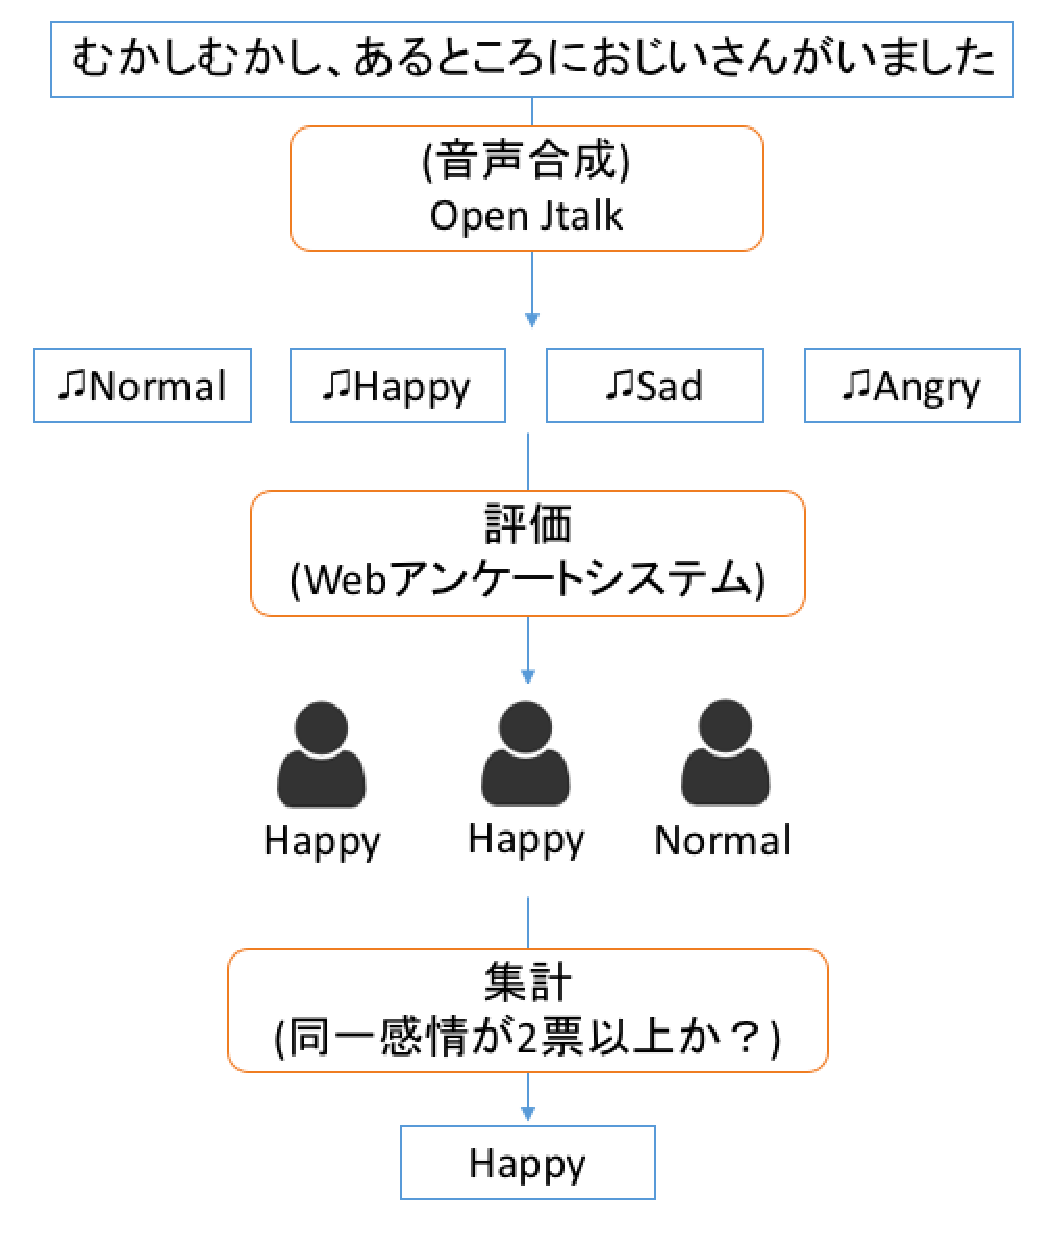
\includegraphics[clip,width=10.0cm]{fig/enquete.eps}
    \caption{学習データの作成手順}
    \label{fig:enquete}
  \end{center}
\end{figure}

\section{物語文章}
本実験では物語データとして,青空文庫\cite{aozora}にある5つの物語を用いる.
青空文庫とは,著作権が消滅した作品や著者が許諾した作品のテキストを公開しているインターネット上の電子図書館である
今回は文体を近づけるために同じ訳者の童話を中心に「白雪姫」,「赤ずきんちゃん」,「浦島太郎」,「ジャックと豆の木」,「ヘンゼルとグレーテル」を用いた.
%TODO 著者などを添えた表

\section{音声データの作成}
\subsection{前処理}

\begin{figure}[hb]
  \begin{center}
    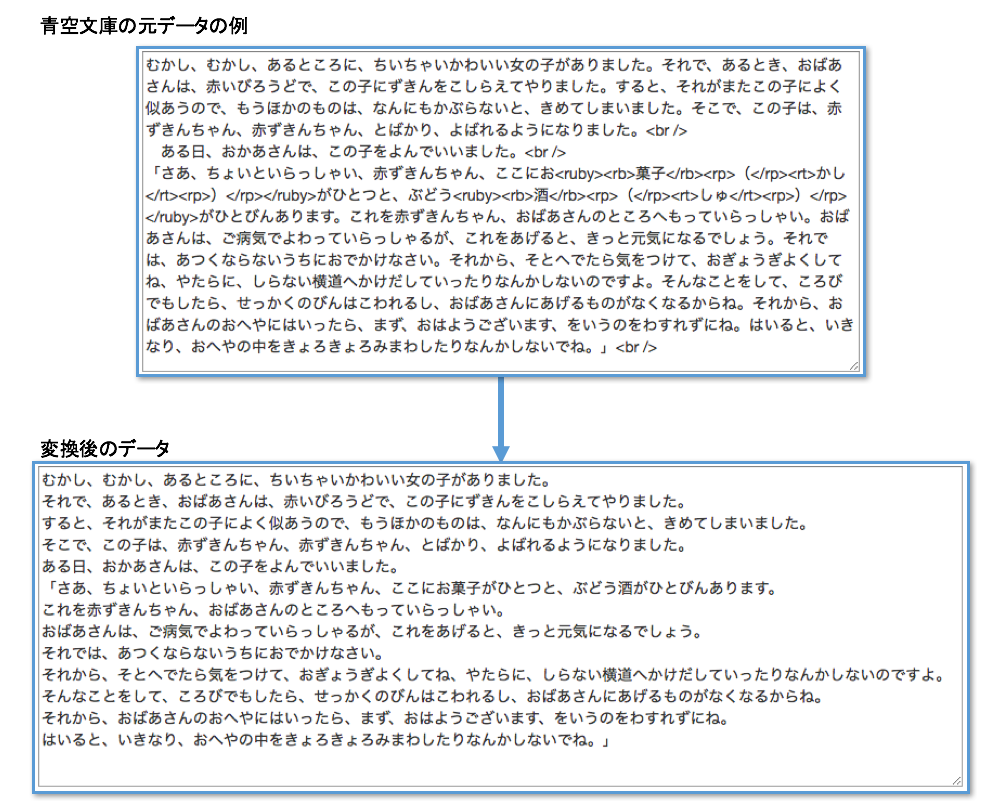
\includegraphics[clip,width=14.0cm]{fig/aozora-convert.eps}
    \caption{青空文庫データの文分割とタグ削除処理}
    \label{fig:aozora-convert}
  \end{center}
\end{figure}


\ref{subsec:divide}で述べたように物語の文章を文に分ける.
朗読システム実現するためにはこの処理も自動化する必要がある.
また,青空文庫の書籍データにはルビや改行といったHTMLタグが挿入されているためこれを除く必要がある.
プログラミング言語Ruby\cite{ruby}を用いて,これらの処理を実装した.
これらの処理の例を\ref{fig:aozora-convert}に示す.

\subsection{音声合成ソフト}
本研究では音声合成にオープンソフトのOpen JTalk\cite{jtalk}を用いる.
Open Jtalkは日本語テキスト向けのHMM型の音声合成のオープンソースのソフトウェアである.
\ref{hmm-emotion}で述べた通りHMM型音声合成手法は少ない学習データで感情表現が可能になっている.
また,再現実験を考慮し広く利用が可能なオープンソースソフトウェアであるOpen Jtalkを用いた.

%TODO バクについて


音声波形データにはMMDAgent\cite{mei}にあるMeiのサンプルを用いた.
この音声波形データは1人の女性の848文の音声サンプルをもとに作成されている.
そのうち,503文は音声波形作成に広く用いられている用いられるATR音素バランス503文\cite{atr}であり,残りのうち215文は普通の発話スタイルで,残る75文は4つの感情(Angry, Bashful, Happy, Sad)の発話スタイルで収録されている.
それゆえ,MMDAgentにはNormal, Angry, Bashful, Happy, Sadの5つの音声波形データが用意されている.
本研究では布目ら\cite{fume}などの研究に従い,このうちのNormal, Angry, Happy, Sadの4つを利用した.


発音辞書にはNAIST Japanese Dictionary\cite{naist}を用いる.

各ソフトウェアの仕様は表\ref{voice-software}に示す.
\begin{table}[ht]
  \begin{center}
  \caption{音声合成のソフトウェア仕様}
  \label{}
  \begin{tabular}{|c|l|}
    \hline
    名称 & バージョン \\ \hline \hline
    Open JTalk & 1.10 \\ \hline
    NAIST Japanese Dictionary & 0.4.3  \\ \hline
    MMDAgent & 1.7 \\ \hline
  \end{tabular}
  \end{center}
\end{table}

\subsection{音声データファイル}
本研究では,前章のOpen JTalkとMeiの音声波形データ等を用いて,一つの文に対して4つの異なる感情表現の音声ファイルを生成する.
この音声ファイルはWAVフォーマット形式で出力される.
WAVフォーマット形式は,非圧縮形式でありリニアPCMのサンプリングデータ用のフォーマットとして扱われる.
Open JTalkの出力ではサンプルレートが48,000Hz,16bps,モノラルのWAVファイルが得られる.
%TODO ↑表にする??

\section{アンケートシステム}

本研究では効率よく学習データを採取するためにWeb上で文に対して感情のラベル付けが行えるシステムを構築した.

\subsection{システムの概要}
\begin{figure}[h]
  \begin{center}
    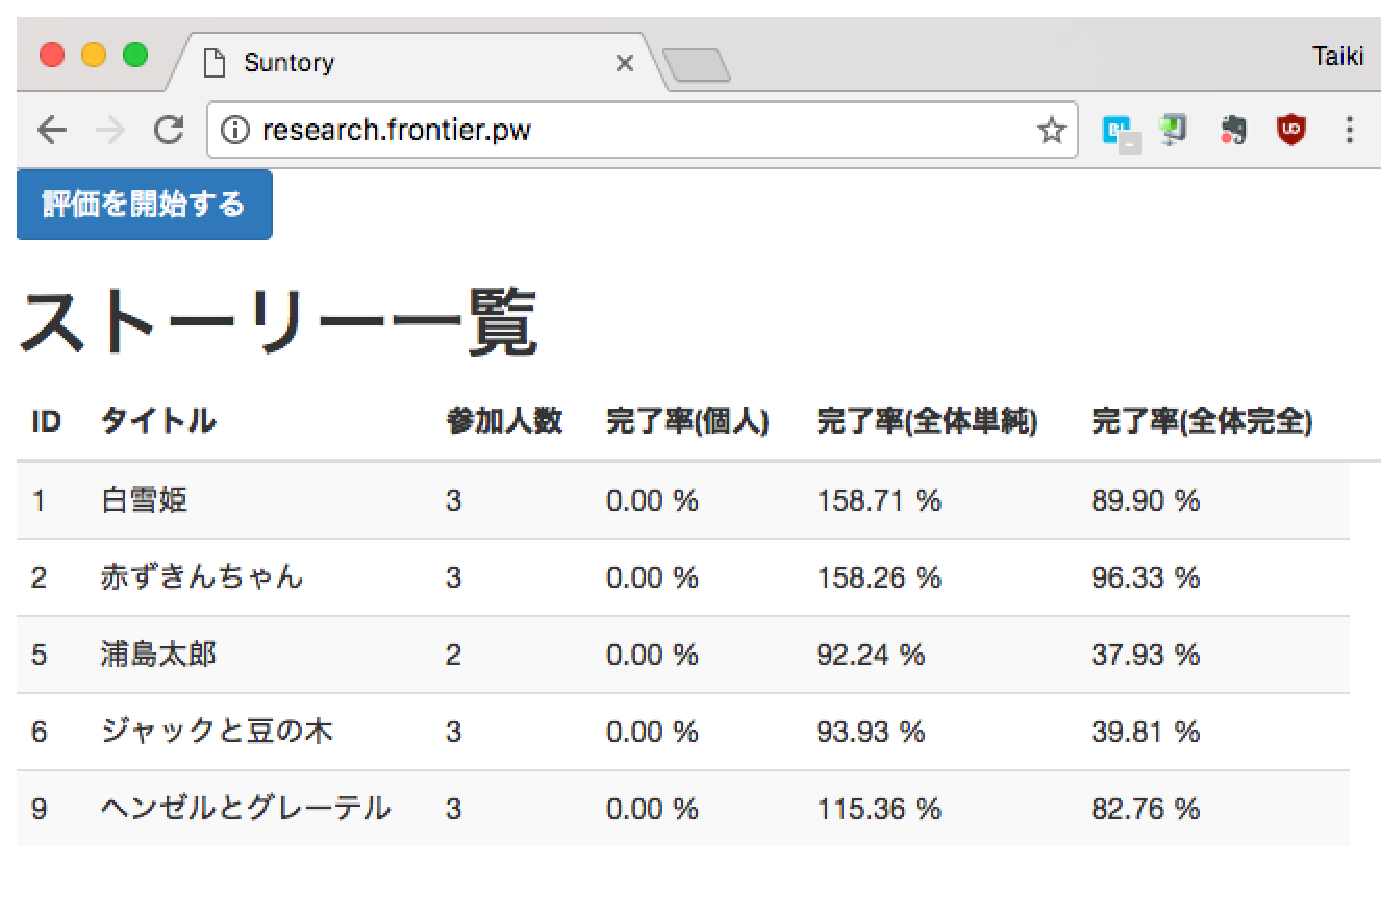
\includegraphics[clip,width=13.0cm]{fig/web-index.eps}
    \caption{WEBアンケートシステム選択画面}
    \label{fig:index-web}
  \end{center}
\end{figure}

\begin{figure}[h]
  \begin{center}
    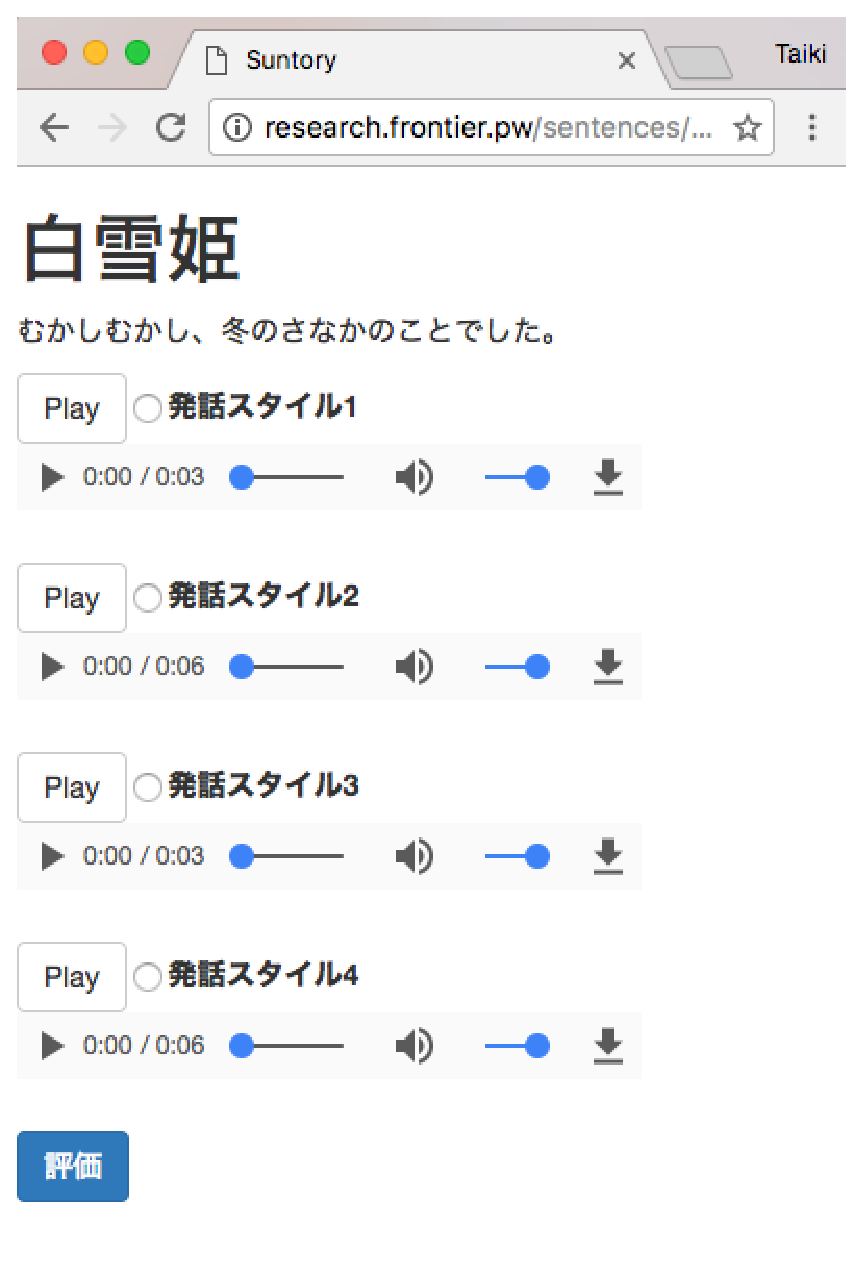
\includegraphics[clip,width=10.0cm]{fig/web.eps}
    \caption{WEBアンケートシステム評価画面}
    \label{fig:web}
  \end{center}
\end{figure}
サインアップもしくはログインを行い評価者は図\ref{fig:index-web}のインデックスページの評価ボタンがから図\ref{fig:web}に示す評価ページに遷移する.
評価ページにおいて後述する評価アルゴリズムに基づいて自動選択された文について評価者は4つの音声それぞれを聞き,内容にもっとも適切(自然)であると思われる感情を1つだけ選択してもらう.
評価ボタンをクリックすると評価はデータベースに保存され,自動選択された別の文の評価ページへと遷移する.

\subsection{システムの利用技術}
WebアプリケーションフレームであるRuby on Rails\cite{rails}を採用し,データベースにはSQlite3\cite{sqlite}を用いた構築した.

評価ページの音声再生部分にはHTML5に定められているWeb Audio APIとaudioタグによる2つの実装を行った.
これは,評価者のブラウザ環境によってはどちらかが使えない場合があるからである.
なお,Playボタンを押すとWeb Audio APIが呼び出されるがこの部分の実装にはJavaScriptを用いた.
これにより,Open JTalkで生成されたWAVファイルが評価自身の端末で再生可能となった.

また,得られた学習データはCSV形式で出力する機能も備えており実用的である.

その他,本システム用いたサーバー機のスペックはソフトウェアの仕様\ref{software}に,表\ref{server}に示す

\begin{table}[ht]
  \begin{center}
  \caption{アンケートシステムのソフトウェア仕様}
  \label{software}
  \begin{tabular}{|c|l|}
    \hline
    名称 & バージョン \\ \hline \hline
    Ruby & 2.3.3p222 \\ \hline
    Ruby on Rails & 4.2.7.1 \\ \hline
    SQLite3 & 3.7.17 \\ \hline
  \end{tabular}
  \end{center}
\end{table}

\begin{table}[ht]
  \begin{center}
  \caption{アンケートシステムのサーバースペック}
  \label{server}
  \begin{tabular}{|c|l|}
    \hline
     名称 & スペック \\ \hline \hline
    マシン &  マウスコンピューター MASTERPIECE i1550PA7-CL-W7\\ \hline
    OS &  CentOS Linux release 7.3.1611 (Core)\\ \hline
    CPU & Intel Core i7-3970X 3.50GHz × 2\\ \hline
    メモリサイズ & 64.0GB \\ \hline
  \end{tabular}
  \end{center}
\end{table}



\subsection{評価アルゴリズム}
被験者には文ごとに各感情のパラメタで合成した音声をそれぞれ聞いてもらい,内容にもっとも適切(自然)であると思われる感情を1つだけ選択してもらう.
しかし,感情は主観的な尺度であるため1人だけの評価では信頼性が低い.
そこで,一文に対して同じ感情の評価が2票集まった時点で評価を確定することとした.
異なる評価が集まった場合はもう1票だけ評価を続け,既存の評価と同じ感情であればその評価で確定することにした.
3票ともに異なる評価が集まった場合には,その文は学習データとしては利用しないこととした.
なお,セリフ文を優先的に評価するように設定した.


\subsection{学習データの収集}
大学生に自身が所有するPCやスマートフォンで,アンケートシステムにアクセスさせ,評価を行わせた.
なお,評価の期限や数は評価者の任意とした.
その他詳細は表\ref{enviroment}に示す.

\begin{table}[ht]
  \begin{center}
  \caption{学習データの収集}
  \label{enviroment}
  \begin{tabular}{|c|l|}
    \hline
    被験者 & 東京理科大学の学部生及び大学院生 \\ \hline
    人数 & 学部生15名,大学院生2名 \\ \hline
    取得期間 & 2017年1月9日〜25日 \\ \hline
    評価取得数 & 2641 \\ \hline
  \end{tabular}
  \end{center}
\end{table}



\section{学習データの概要}
学習データの概要を表\ref{sentence-count}と表\ref{emotion-count}に示す.

全体で評価が確定したものは全体で69.8\%であった.
セリフは全体の33.21\%であり,セリフの評価完了率は81.04\%であった.
表\ref{emotion-count}の通り,Normal以外の感情はセリフに多く含まれており,セリフの方が感情豊かであり,それ以後の文はNormalであることが多いことがわかる.

\begin{table}[ht]
 \centering
  \caption{学習データ(物語別)}
  \vspace{0.3\baselineskip}
  \scalebox{0.8}{
  \begin{tabular}{|c|c|c|} \hline
    タイトル & 文数(セリフ) & 評価確定数(セリフ) \\ \hline \hline
    白雪姫 & 287 (90) & 258 (86)   \\ \hline
    赤ずきんちゃん & 109 (54) & 108 (54)   \\ \hline
    浦島太郎 & 206 (48) & 78 (26)   \\ \hline
    ジャックと豆の木 & 206 (49) & 78 (26)   \\ \hline
    ヘンゼルとグレーテル & 319 (114) & 260 (90)   \\ \hline\hline
    合計 & 1096 (364) & 765 (283) \\ \hline
  \end{tabular}
  }
  \label{sentence-count}
\end{table}

\begin{table}[ht]
 \centering
  \caption{学習データ(感情別)}
  \vspace{0.3\baselineskip}
  \scalebox{0.90}{
  \begin{tabular}{|c|c|c|} \hline
    感情 & 全文 & セリフのみ  \\ \hline \hline
    Normal & 459  & 63  \\ \hline
    Happy & 134 & 110 \\ \hline
    Sad & 99  & 60  \\ \hline
    Angry & 73  & 50  \\ \hline \hline
    合計 & 765 &  283 \\ \hline
  \end{tabular}
  }
  \label{emotion-count}
\end{table}

\section{本章のまとめ}
本章では,本研究に用いるデータセットの説明や収集方法,アンケートシステムの詳細について説明した.



